\newpage
\section{整体架构}
\label{sec:architecture}

\begin{figure}[htbp]
	\centering
	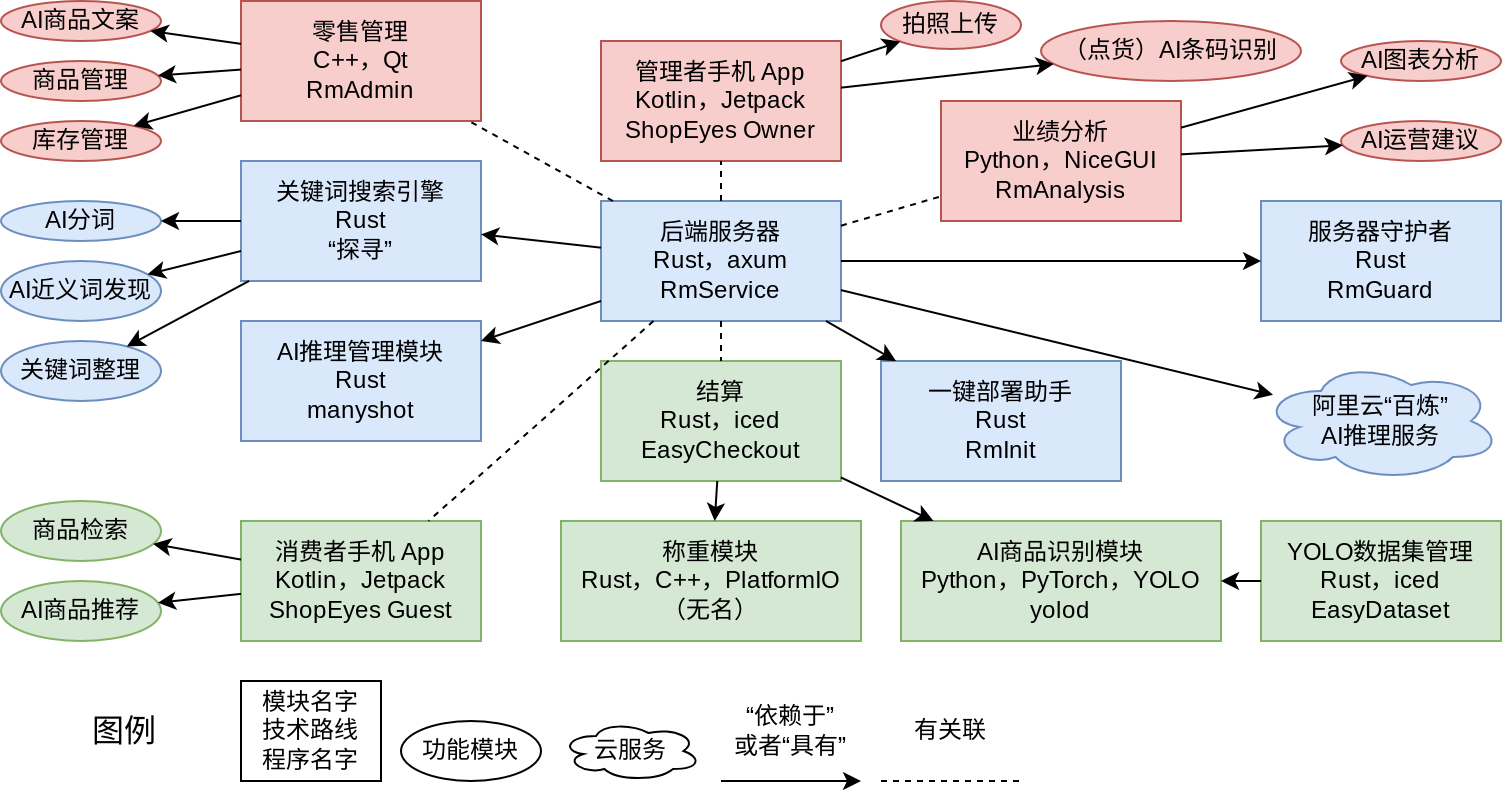
\includegraphics[width=0.8\textwidth]{./imgs/structure2.png}
	\caption{本设计的系统架构图示:其中蓝色部分为服务端,红色部分为商家端、绿色部分为顾客端。图例(不同形状的各自意义)位于图像下侧。}
	\label{fig:structure2}
\end{figure}

本设计的系统架构如图 \ref{fig:structure2} 所示,而从图像中不难看出,该系统整体上呈现出客户端-服务器模式的结构,其中客户端部分分为面向零售行业从业者的商家端和面向最终消费者的顾客端。

\subsection{服务端}

本设计中对服务端功能的期望主要有如下几点:

\begin{itemize}
    \item 高性能的HTTP API服务器
    \item 商品、库存、订单等运营资料的增删改查
    \item 高性能、效果良好的智能商品搜索
    \item AI大语言模型推理托管
\end{itemize}

实际部署的情况下,服务器可能需要在短时间内处理来自大量客户端应用程序的服务请求,比如营业高峰期来自许多客人的商品检索、询问AI助手索取导购建议的请求,因此服务器本身的效率必须纳入设计的考虑之中。基于这样的考虑,该设计采用Rust语言进行开发。Rust是比较流行的一门强调内存安全的系统编程语言,利用这门语言,服务器的代码执行效率有充足的优化机会,并且开发的便利性得到了一定保证。为了充分利用大部分部署环境都将会具备的多处理器的对称并行处理(SMP)执行环境,服务器内主要采用由tokio第三方库驱动的异步开发的技术手段。为了实现服务器与客户端的有效、高效、泛用性强的信息双向传输,采用通过(商铺内部)局域网的HTTP。为了与总体的技术选择相统一,采用依托并行计算技术开发的axum HTTP服务器框架。

服务器需要能实际储存并处理在零售运营过程中需要的各种数据。为了满足这个期望,该设计中采用基于SQLite关系数据库引擎的rqlite分布式关系数据库管理软件作为原始数据存储、查询和管理的手段。为了提供统一可靠的开发接口,rqlite服务器将只面向服务器软件开放,而客户端任何对实际业务数据的访问都必须通过服务器对其结构化、统一化的封装。

为了实现在众多商品中快速找到顾客所需,服务器需要具备通过(顾客提供的)一段可能和商品本身文字内容不尽相同的搜索语句对商品进行匹配的功能。市面上常见的如Apache Lucene、Elasticsearch等各种相关产品与该设计的相关理念并不匹配:因为较为复杂而不适合在该设计所期望的低成本设备上部署;对中文没有比较深入的优化,并且搜索对象仅限于搜索目标中出现过的字词。为了解决这个问题,该设计中包含一个由多种人工智能技术驱动的,高效、高匹配率、简明易用的中文特化搜索引擎“探寻”。

鉴于该项目中多处利用到了大语言模型,若是服务器可以向各个客户端软件提供统一的推理接口,将不同模型、不同服务商的区别消除,将有利于项目的整体可用性、可维护性。因此,服务器提供一个专门开发的的推理模块,具备单次推理(“oneshot”)、多次尝试(“manyshot”)和有状态多轮对话管理等功能。

\subsection{商家端}

本设计中对商家端功能的期望主要有如下几点:

\begin{itemize}
    \item 高性能、便于使用的用户界面
    \item 功能丰富、易于操作的商品、库存管理界面
    \item 完整的销售数据查询界面
    \item 业绩图表生成、展示界面
    \item 业绩图表AI智能分析、运营建议
    \item AI条码识别点货
    \item AI商品文案自动生成、批量生成
    \item 商品识别数据集创建和修改
    \item 从手机上传用于商品的图片
\end{itemize}

为了在普通的计算机上高效管理营业资料,商家端需要一套对系统要求较小的、对键盘鼠标操作较为友好的,对屏幕尺寸需求灵活的用户界面。基于这样的缘由,该设计的商家桌面端应用程序采用Kotlin作为业务逻辑开发语言以最大化开发效率,进而采用受到工业界广泛采用的Qt Widgets应用程序开发框架在Java、Kotlin语言上的实现Qt Jambi。

在实际操作的情况下,经营者不可避免地将需要对各类数据进行条件细致的筛选。为了满足这样的需要,商家桌面端应用程序为多种不同零售资料的查询准备了既功能丰富,又简单易懂的图形化高级搜索条件拟写工具。

将销售数据按表格列出是简单易行的,但这样的数据展示方式往往无法满足营业者的营业数据分析的需要,图表可以更好地呈现数据之中潜在的结构性和规律性。为了实现这样的功能,本设计采用业界惯用的Python语言作为数据分析的主要语言,利用HTTP API与基于Rust的服务器进行通讯,并采用pandas、numpy等数据科学库展开数据整理工作,利用matplotlib库进行图形的绘制。为了简化开发过程,图表部分的用户界面同样采用Python编写,同时选择NiceGUI用户界面框架实现与上述第三方库更高的整合度。

为了减轻零售从业者观察图形规律的压力,该设计利用来自阿里云“百炼”AI推理服务的多个AI模型,针对不同类型、复杂程度的营业数据图表进行“先观察后思考”的“接力式”智能分析报告编写或者“边观察边思考”的快速图形规律总结,向从业者提供详尽准确的数据分析。

业务资料中的商品图片较为特殊,在手机设备上处理可能相比在桌面型计算机上更加便捷。因此,该项目采用Jetpack Compose安卓应用程序开发框架实现面向商家的管理用应用程序。利用该应用程序营业者可以较为简单地将手机中的照片或现场拍摄的照片上传到服务器中。

实体零售行业常常无法避免对仓库中、货架上产品进行审计(统计),以此确认实际产品数量与系统中库存数量对应关系的需要,而手工记录并比照的方法费时费力并且容易出现错误。因此,该设计的移动商家端应用程序采用谷歌MLKit的AI条码识别功能开发了利用手机自带摄像头的AI条码识别并记录、上传的功能。

为了简化用于智能结算房屋中的商品识别模型的训练工作,该项目具备利用Rust和iced用户界面框架开发的数据集创建和修改功能。数据集准备的过程分为“类别规划”“图片采集”和“图片管理”三个连贯的部分。从业者能够先根据实际的需要在应用程序中输入需要的商品种类,再利用智能商品识别对应的摄像设备进行数据集中图片的采集,最后在采集的图片中筛选出质量较高者。

\subsection{顾客端}

本设计中对顾客端功能的期望主要有如下几点:

\begin{itemize}
    \item 美观大方、便于使用的用户界面
    \item 推荐商品浏览
    \item 商品检索和详情浏览
    \item AI导购多轮对话商品推荐
    \item 基本商品结算
    \item AI商品识别-计重结算
\end{itemize}

为了最大程度提高消费者获取商品信息的便利程度,增强新零售购物体验,该项目采用Jetpack Compose开发面向消费者的用于浏览商品情况的应用程序。应用程序分为“推荐”“搜索”和“询问AI”三个板块,分别通过不同的用户界面、不同的对服务器API的请求方式来实现相应的功能。其中推荐功能展示由从业人员在商家端预先设置的一系列推荐商品,而搜索功能顾名思义。

另一个功能是“询问AI”。在该功能界面下,用户可以通过屏幕底部的搜索框输入需要向AI询问的导购相关问题,用户输入的问题将会经由服务器中转发送到后端预先指定的推理服务和选择的大模型。在获取输出之后,顾客端应用程序会利用AI的答复再次利用AI进行关键词的提取,进而利用归纳得出的关键词进行对商品的检索,进而实现对用户推荐相关的商品的功能。

为了同时满足店员辅助结算和消费者自主结算的需要,该项目需要提供一个用于结算设备的简洁明了的用户界面。因此,该设计采用Rust语言及iced用户界面开发框架设计开发结算用用户界面。用户可以利用通过人体工学输入设备(HID)方式连接到结算设备的激光条码扫描设备来输入任何按件结算的商品。

某些零售细分领域所提供的商品(如生鲜蔬果、熟食等)是按重量结算的,需要称重才能获取实际价格,并且按实际情况有可能商品表明无法粘贴对应的条形码(比如肉类),需要其他手段辅助才能确定商品的具体类型。为了解决这样的问题,本设计利用YOLO图像分类模型,结合前文提及的商家端数据集管理工具,开发AI智能商品识别算法,用以简化计重商品结算流程。